\documentclass[10pt,twocolumn,letterpaper]{article}

\usepackage{cvpr}
\usepackage{times}
\usepackage{epsfig}
\usepackage{graphicx}
\usepackage{amsmath}
\usepackage{amssymb}

% Include other packages here, before hyperref.

% If you comment hyperref and then uncomment it, you should delete
% egpaper.aux before re-running latex.  (Or just hit 'q' on the first latex
% run, let it finish, and you should be clear).
\usepackage[breaklinks=true,bookmarks=false]{hyperref}

\cvprfinalcopy % *** Uncomment this line for the final submission

\def\cvprPaperID{****} % *** Enter the CVPR Paper ID here
\def\httilde{\mbox{\tt\raisebox{-.5ex}{\symbol{126}}}}

% Pages are numbered in submission mode, and unnumbered in camera-ready
%\ifcvprfinal\pagestyle{empty}\fi
\setcounter{page}{4321}
\begin{document}

%%%%%%%%% TITLE
\title{Report of latest found}

\author{Ruzhuo Wang\\
	%University of California, Riverside\\
	%Institution1 address\\
	{\tt\small rwang085@ucr.edu}
	% For a paper whose authors are all at the same institution,
	% omit the following lines up until the closing ``}''.
	% Additional authors and addresses can be added with ``\and'',
	% just like the second author.
	% To save space, use either the email address or home page, not both
	\and
	%Second Author\\
	%Institution2\\
	%First line of institution2 address\\
	%{\tt\small secondauthor@i2.org}
}

\maketitle
%\thispagestyle{empty}



%%%%%%%%% BODY TEXT
\section{What the paper do }
\subsection{Average forward time estimation of convolutional layer}
Given the matmul of $[n\times k]$ and $[k\times m]$ (the number of FLOPs is
$n\times m\times k$) performed by a CONV layer, $n$ is the number of kernels, $k$
is the size of a kernel in 3D ($width\times height\times depth$, where depth is
the number of input feature maps), and $m$ is the spatial size ($width\times height$) of output feature maps. \par
I find that the average forward time is linearly related to FLOPs ($n\times m\times k$) 

\begin{figure}[h]
	\begin{center}
		
		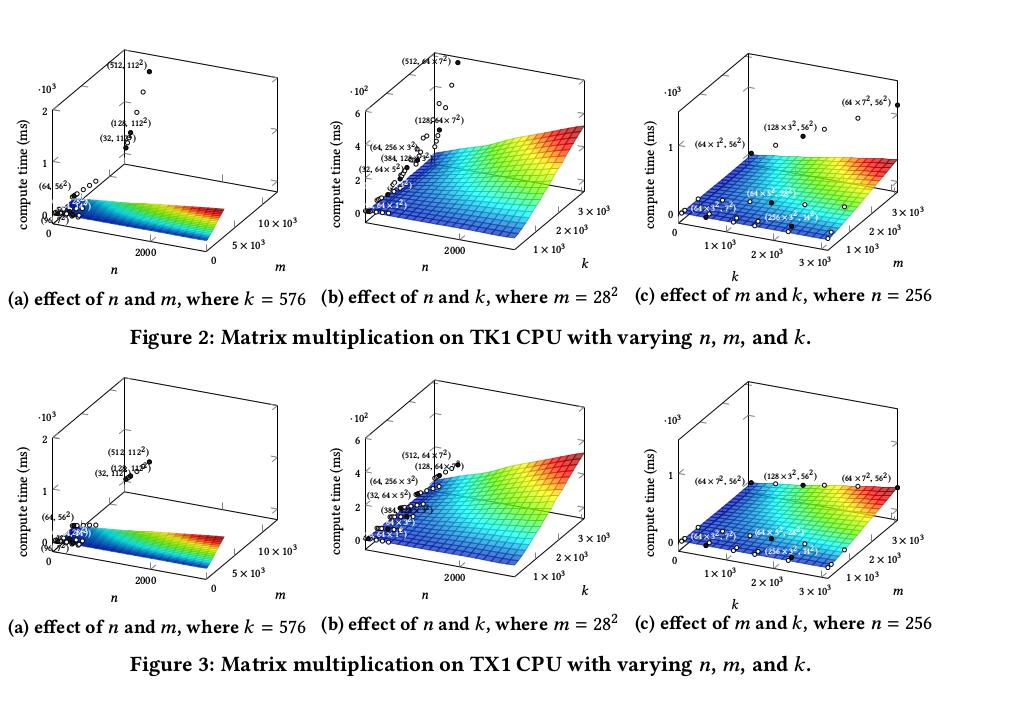
\includegraphics[width=1\linewidth]{they1.png}
	\end{center}
	\caption{The data they provide}
	\label{fig:long1}
	\label{fig:onecol1}
\end{figure}
\subsection{Memory}
The memory requirement to run a CNN comes from three major
sources: $(i)$ the memory that holds the parameters of the CNN; $(ii)$
the memory that stores intermediate data of the CNN; and $(iii)$ the
workspace for computation.
%-------------------------------------------------------------------------
\section{What I do }
\subsection{Average forward time estimation}
\subsubsection{For fully connected layer}
The average forward time for a fc(fully connected) layer is determined by the number of nodes for adjacent layers, $e.g.$ one fc layer has $m$ nodes, the adjacent fc layer has $n$ nodes, then the average forward time is linearly related to $m\times n$. \par
In Figure 2, '1k x 1k x 5' means fc1 layer has 1000 nodes, the adjacent layer for fc1 is fc2 and fc2 has 1000 nodes, the adjacent layer for fc2 is fc3 and fc3 has 5 nodes.
\begin{figure}[h]
	\begin{center}
		
		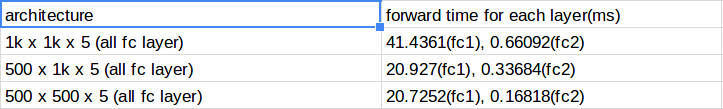
\includegraphics[width=1\linewidth]{mine1.png}
	\end{center}
	\caption{The raw data I have for fc layer forward time}
	\label{fig:long2}
	\label{fig:onecol2}
\end{figure}

\subsubsection{For convolutional layer}

Assume the output number is $x$, kernel size is $y_1\times y_2$, stride is $z$, the input batch size is $k$, input height is $m$, input width is $n$, input channel is $c$, then the average forward time should be linearly related to:
\[k\times x\times c\times y_1\times ceil(\frac{m\times floor(\frac{y_1}{2})\times 2}{z})\times y_2\times ceil(\frac{n\times floor(\frac{y_2}{2})\times 2}{z}) \]
\begin{figure}[h]
	\begin{center}
		
		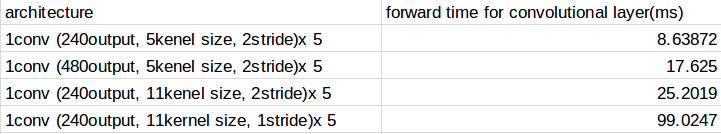
\includegraphics[width=1\linewidth]{mine2.png}
	\end{center}
	\caption{The raw data I have for convolutional layer forward time}
	\label{fig:long3}
	\label{fig:onecol3}
\end{figure}


\subsection{Memory}
\begin{figure}[h]
	\begin{center}
		
		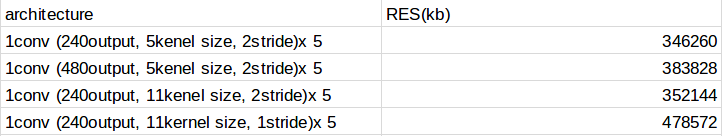
\includegraphics[width=1\linewidth]{mine3.png}
	\end{center}
	\caption{The raw data I have for convolutional layer memory}
	\label{fig:long4}
	\label{fig:onecol4}
\end{figure}
I only have the raw data for memory estimation.


%-------------------------------------------------------------------------


\end{document}
